\documentclass[12pt,a4paper]{scrartcl}
\usepackage[utf8]{inputenc}
\usepackage{graphicx}
\usepackage{ngerman}
\usepackage{url}
\usepackage{amsmath}
\usepackage{caption}
\usepackage{wrapfig}
\usepackage{eurosym}
\usepackage{biblatex}
\usepackage{url}
\usepackage{color}
\usepackage{listings}
\usepackage{hyperref}
\usepackage[table]{xcolor}
\linespread{1.4}

\definecolor{mygreen}{rgb}{0,0.6,0}
\definecolor{mygray}{rgb}{0.5,0.5,0.5}
\definecolor{mylightgray}{rgb}{0.7,0.7,0.7}
\definecolor{mylightergray}{rgb}{0.9,0.9,0.9}
\definecolor{mymauve}{rgb}{0.58,0,0.82}

\let\origitemize\itemize
\def\itemize{\origitemize\itemsep0pt}

\lstset{ 
  backgroundcolor=\color{white},   
  basicstyle=\ttfamily\footnotesize,          
  breakatwhitespace=false,         
  breaklines=true,  
  commentstyle=\color{mygreen}, 
  escapeinside={\%*}{*)}, 
  extendedchars=true,             
  keepspaces=true,                 
  keywordstyle=\color{blue},
  language=Octave,
  numbers=left,                   
  numbersep=15pt,                  
  numberstyle=\tiny\color{mygray}, 
  showspaces=false,                
  showstringspaces=false,          
  showtabs=false,                  
  stringstyle=\color{mymauve},
  tabsize=2,
  title=\lstname,
  captionpos=b
}

\renewcommand*\lstlistingname{Codebeispiel}    %Rename Listings

\renewcommand*\thesection{\arabic{section}}

\makeatletter
\renewcommand\subparagraph{\@startsection{subparagraph}{5}{\parindent}%
    {3.25ex \@plus1ex \@minus .2ex}%
    {0.75ex plus 0.1ex}% space after heading
    {\normalfont\normalsize\bfseries}}
\makeatother

\begin{document}
\title{Praktikum Data Mining}
\subtitle{Energieverbrauch und CO2-Emmisionen \newline Vorhersage und Clustering auf Finanzdaten}
\author{Oliver Fesseler \and Maria Florus\ss \and Stefan Seibert \and  Daniel Grie\ss haber}
\maketitle
\newpage
\tableofcontents
\newpage

\part*{Energieverbrauch und CO\textsubscript{2}-Emmission}

\section*{Datenverwaltung und Statistik}
\subsection*{Einlesen der Daten, Hinzuf\"ugen der GPS Koordinaten, Abspeichern in neuer Datei}
Bei der Umsetzung der Aufgaben haben wir mit verschiedenen Darstellungsformen der Daten experimentiert. Im ersten Plot fallen vor allem die Vielverbraucher einzelner Energieformen auf. Beim zweiten Plot k\"onnen die verschiedenen Energiemixe pro Land direkt miteinander verglichen werden, da sie alle im selben Ma\ss stab nebeneinander dargestellt werden.

\subparagraph{Frage: Ausgehend von der implementierten Visualisierung des Energieverbrauchs der L\"ander: Nennen Sie die 3 Ihrer Meinung nach interessantesten Beobachtungen.}

\begin{enumerate}
\item Durch die wenigen Industriel\"ander mit signifikant h\"oherem Energieverbrauch, wie China oder die USA, wird der Plot so verzerrt, dass die L\"ander mit durchschnittlichem Verbrauch im Plot so gestaucht werden, dass sie kaum zu erkennen sind. Dies k\"onnte behoben werden, wenn die Daten mit den Einwohnerzahlen aller L\"ander normalisiert werden w\"urden. So k\"onnte der Pro-Kopf-Verbrauch berechnet werden, was einen besseren Vergleich der einzelnen L\"ander bietet.
\item Dieses Prinzip wird klar bei der Betrachtung von China und Indien, die von der Einwohnerzahl her vergleichbar sind (China 1,3 Mrd., Indien 1,2 Mrd.\footnote{Stand 2012, Quelle: Wikipedia}). China zeigt einen weitaus h\"oheren Verbrauch als Indien an den in beiden L\"andern h\"aufigen Energieformen Kohle und \"Ol.
Zus\"atzlich w\"aren noch andere Normalisierungsfaktoren interessant:
\begin{itemize}
\item Bruttoinlandsprodukt
\item Au\ss enhandelsstatistik oder Export der L\"ander in US\$
\item Technologieindex
\end{itemize}
\item Die zwei L\"ander mit dem h\"ochsten Energieverbrauch sind China und die USA. Dies f\"allt bei der Betrachtung des Gesamtenenergieverbrauchs auf. Bei der Betrachtung des Verbrauchs einzelner Energieformen wirkt es als sei China durch seinen hohen Kohleverbrauch weit vor den USA.
\end{enumerate}

\subparagraph{Abgabe: Relevante Dateien}
\begin{itemize}
\item \lstinline{energy_consumption_per_country.py} und \lstinline{energy_consumption_per_country_V2.py} \\- Implementierung Aufgabe 2.1.2: 1) - 2)
\item \lstinline{energy_consumption_per_country.pdf} \\- Ausgabe des Skripts \lstinline{energy_consumption_per_country.py} 
\item \lstinline{energy_consumption_per_country_V2.pdf} \\- Ausgabe des Skripts \lstinline{energy_consumption_per_country_V2.py}
\item \lstinline{appendGeoCoordinates.py} \\- Implementierung Aufgabe 2.1.2: 3) - 5)
\item \lstinline|EnergyMixGeo.csv|  \\- Ausgabe des Skripts \lstinline{appendGeoCoordinates.py}
\end{itemize}





\subsection*{Statistik der Daten}


\subparagraph{Frage: Erkl\"aren Sie s\"amtliche Elemente eines Boxplot (allgemein). }
\begin{figure}[!h]
\centering
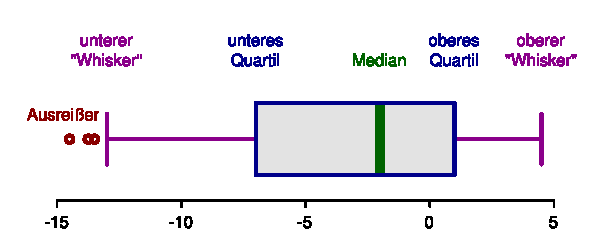
\includegraphics[width=\textwidth]{Plots/Elements_of_a_boxplot.svg}
\end{figure}


\subparagraph{Abgabe: Relevante Dateien}
\begin{itemize}
\item
\end{itemize}


\end{document}